
%(BEGIN_QUESTION)
% Copyright 2006, Tony R. Kuphaldt, released under the Creative Commons Attribution License (v 1.0)
% This means you may do almost anything with this work of mine, so long as you give me proper credit

Denne illustrasjonen viser en portstyrt globeventil med {\it lineer} reguleringskarakteristikk:

$$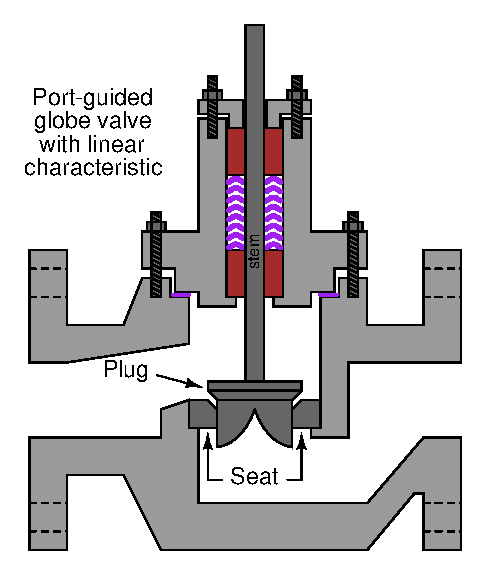
\includegraphics[width=8cm]{i00060x01.eps}$$

Beskriv {\it og} skisser hva som ma endres i denne ventilen for a gi den en {\it likeprosent} reguleringskarakteristikk.

\vfil

\underbar{file i00060}
\eject
%(END_QUESTION)





%(BEGIN_ANSWER)

Dette er et vurdert sporsmal -- ingen svar eller hint gis!

%(END_ANSWER)





%(BEGIN_NOTES)

For a konvertere en {\it lineer} ventilplugg til en {\it likeprosent} ventilplugg ma vi omforme pluggen slik at den ``apner tregere'' enn for.  Med andre ord ma reguleringskurven omformes slik at den gir en mindre apning ved lave spindelposisjoner enn for, samtidig som den apner like mye som for nar pluggen er fullt trukket tilbake fra setet.

Portstyrte globeventilplugger forblir alltid i kontakt med seteringen for styring og stotte.  I motsetning til spindelstyrte plugger som trekkes helt ut av setet, har en portstyrt plugg alltid en del av seg selv inn i seteboringen.  Dette betyr at den delen av pluggen som struper ved lave spindelposisjoner ligger naer tetningsflaten pa den ovre delen av pluggen.  Med andre ord er toppen av kurven der strupingen skjer nar ventilen akkurat begynner a apne.

Derfor, for a fa denne ventilpluggen til a apne ``tregere'' enn for, ma den buede utsparingen begynne smalere enn for, og deretter apne seg aggressivt til full bredde mot bunnen:

$$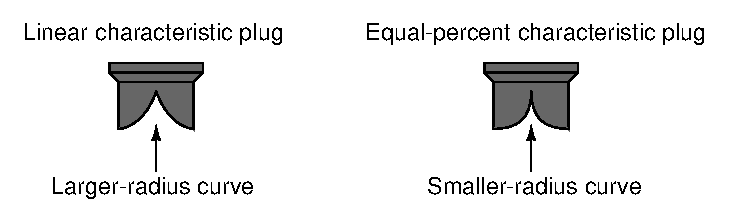
\includegraphics[width=15.5cm]{i00060x02.eps}$$

%If this new equal-percentage plug shape does not present as full an opening at the 100\% position as it did when shaped for a linear characteristic, we could trim the plug to be shorter (and therefore be 

%INDEX% Final Control Elements, valve: equal-percentage characteristic

%(END_NOTES)



